\documentclass{article}
\usepackage[T1]{fontenc}

\usepackage{graphicx}
\usepackage{listings}
\begin{document}

\title{FOSS Lab Report}
\author{Gokul K\\[2\baselineskip]
Roll Number: 21\\[2\baselineskip]}
\date{06 February 2020}

\maketitle

\setcounter{section}{21}
\section{Awk Scripting III}
\subsection{Aim}

Write an awk script to find out total number of books sold in each discipline
 as well as total book sold based on the given table\newline
electrical 34\newline
mechanical 67\newline
electrical 80\newline
computers 43\newline
mechanical 65\newline
civil 198\newline
computers 64\newline

\subsection{Source Code}
\begin{verbatim}
    #! /bin/awk -f

    # Write an awk script to find out total number of books sold in each discipline
    # as well as total book sold based on the given table
    # electrical 34
    # mechanical 67
    # electrical 80
    # computers 43
    # mechanical 65
    # civil 198
    # computers 64
    
    {
        totalByDisc[$1] += $2
        total += $2
    }
    
    END{
        print "Dept: Total"
        print "----------"
    
        for(i in totalByDisc){
            print i ": " totalByDisc[i]
        }
    
        print "----------"
        print "Total: " total
    }
\end{verbatim}

\subsection{Output}
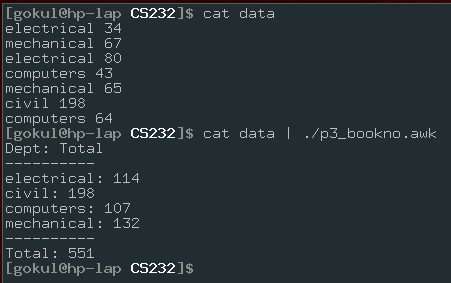
\includegraphics[width=0.9\textwidth]{img/p22.png}\newline

\subsection{Result}
The above program is run on Manjaro Linux running GNU Awk 5.0.1. 
Each query is checked and output is verified
\end{document}